\chapter{Evaluatie}
\label{ch:evaluatie}
In dit hoofdstuk bespreken we de bekomen resultaten. 
Per grafiek wordt het verschil tussen een correct uitgevoerde bench press en een foutief uitgevoerde bench press geanalyseerd. 
Hierbij wordt telkens gekeken naar de variaties in hoeken tussen verschillende lichaamssegmenten. 
Vervolgens wordt besproken in hoeverre deze verschillen overeenkomen met de verwachtingen.

\section{Bench Press}
\subsection{Onvolledige uitvoering}

De grafiek in Figuur~\ref{fig:incomplete_rep} toont de verschillen in hoeken tussen een correcte uitvoering en een uitvoering waarbij de oefening niet volledig werd afgemaakt. 
Zoals verwacht zien we hier vooral verschillen bij de schouder-elleboog-pols-hoek (lichtblauw), die naarmate de oefening vordert niet de volledige extensie bereikt. 
Dit komt overeen met de observatie dat de gebruiker de stang niet volledig tot de borst laat zakken.

\begin{figure}[H]
    \centering
    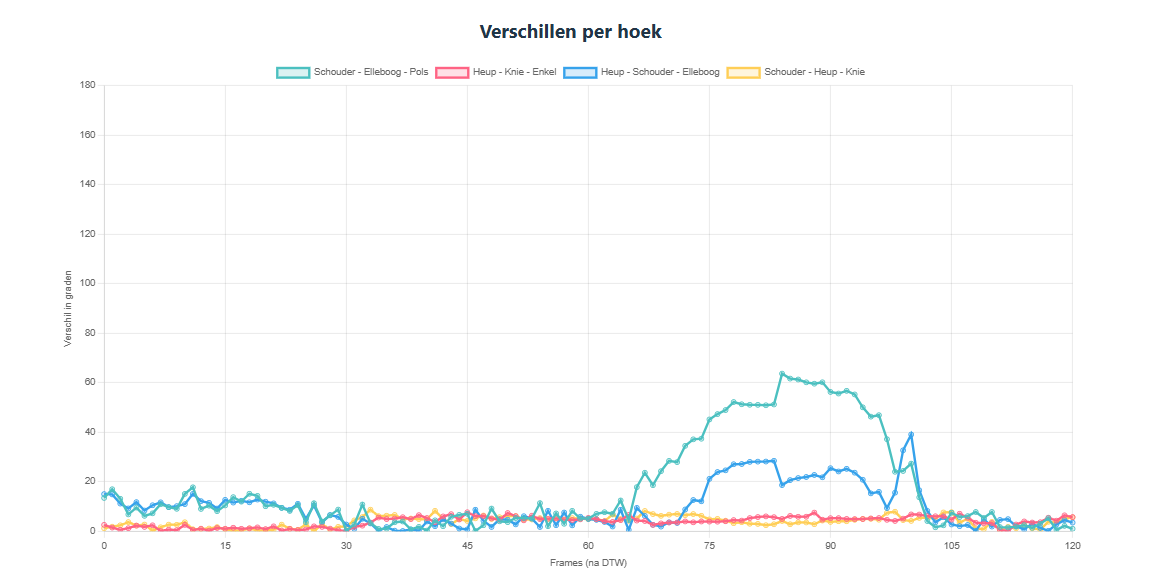
\includegraphics[width=0.9\textwidth]{bench_incomplete_rep.png}
    \caption{Verschillen per hoek bij een incomplete rep}
    \label{fig:incomplete_rep}
\end{figure}

\subsection{Gebogen rugpositie}

De grafiek in Figuur~\ref{fig:arched_back} toont significante afwijkingen in zowel de heup-schouder-elleboog-hoek (donkerblauw) als de heup-knie-enkel-hoek (oranje) bij een bench press met overmatige rugkromming. 
De heup-knie-enkel-hoek toont een constante afwijking van 15°-20°, wat wijst op onvoldoende stabilisatie vanuit de onderste extremiteiten. 
Dit duidt op compensatie door een overdreven holle rug, wat het risico op lage rugbelasting verhoogt.

\begin{figure}[H]
\centering
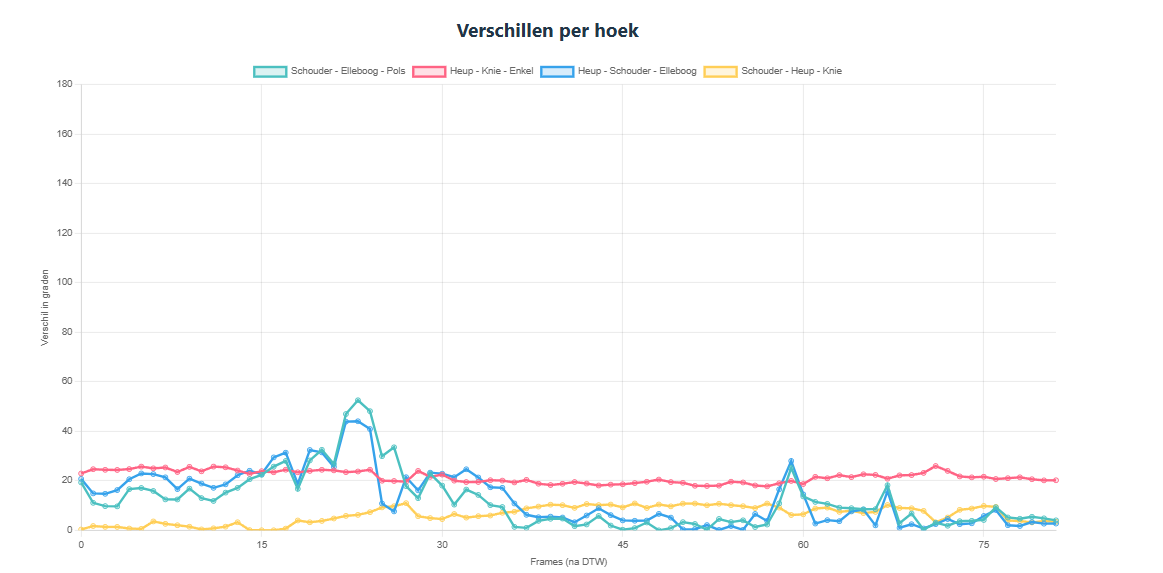
\includegraphics[width=0.9\textwidth]{bench_arched_back.png}
\caption{Hoekverschillen bij bench press met gebogen rug}
\label{fig:arched_back}
\end{figure}

\subsection{Incorrecte elleboogpositie}

Figuur~\ref{fig:bad_elbows} laat zien wat er gebeurt bij een bench press waarbij de ellebogen te ver naar buiten staan. 
Normaal horen de ellebogen ongeveer onder een hoek van 75° ten opzichte van het lichaam te blijven, maar hier zien we onnatuurlijke schommelingen in de armhoek (lichtblauwe lijn).

Ook de houding van de bovenrug (groene lijn) ziet er stijver uit dan normaal. 
Dit komt omdat het lichaam probeert te compenseren voor de verkeerde elleboogstand. 
Door deze foute houding komt er te veel druk op de schouders te staan, wat het risico op blessures verhoogt.

\begin{figure}[H]
\centering
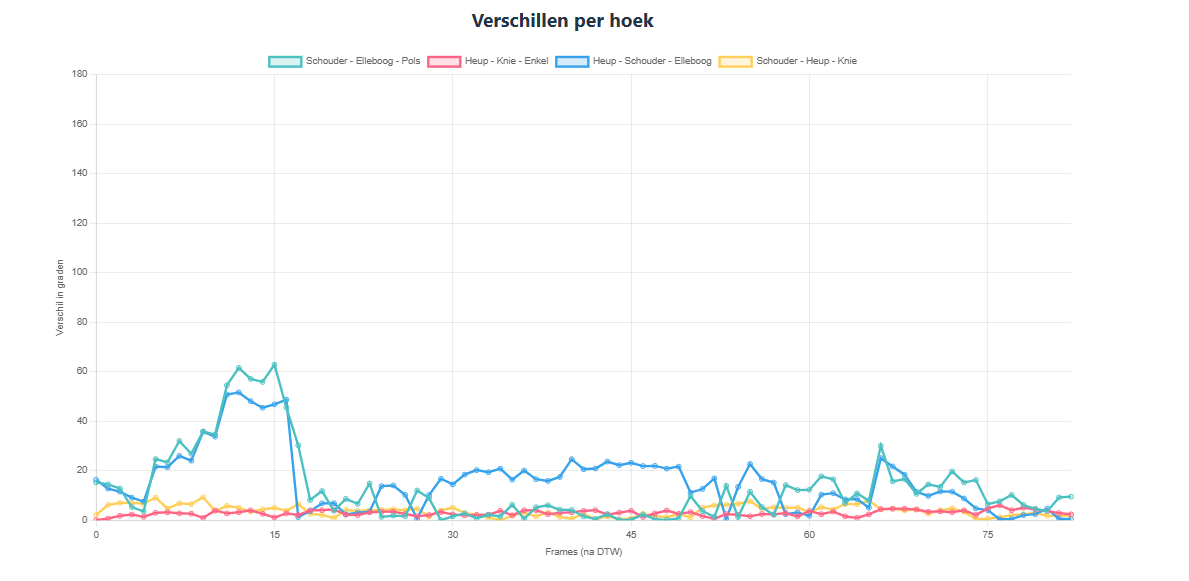
\includegraphics[width=0.9\textwidth]{bench_bad_elbows_comparison.png}
\caption{Ellebooghoekvergelijking bij foutieve techniek}
\label{fig:bad_elbows}
\end{figure}

\section{Deadlift}
\subsection{Te brede voetstand bij deadlift}

Figuur~\ref{fig:deadlift_stance_wide} toont de resultaten van een deadlift met een te brede stand.
De opvallendste verandering is opnieuw in de heup-knie-enkel-hoek (roze lijn), met een geleidelijke toename in de middenfase van de beweging (rond frame 70). 
De verschillen in schouder-heup-knie (gele lijn) blijven laag, wat suggereert dat de bovenlichaampositie correct blijft.
Echter, de bredere stand kan biomechanisch inefficiënt zijn voor sommige lichaamsbouwtypes en verhoogt het risico op heupblessures of overbelasting van de lies.

\begin{figure}[H]
\centering
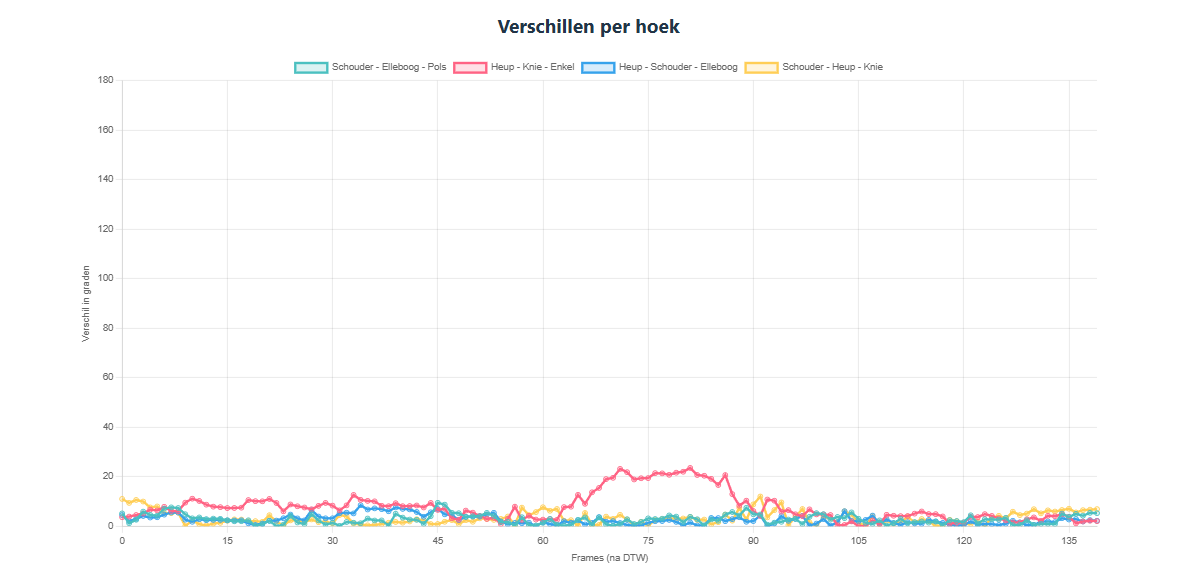
\includegraphics[width=0.9\textwidth]{deadlift_stance_too_wide.png}
\caption{Hoekverschillen bij deadlift met te brede voetstand}
\label{fig:deadlift_stance_wide}
\end{figure}

\subsection{Foute rugpositie tijdens deadlift}

Zoals weergegeven in Figuur~\ref{fig:deadlift_bad_back}, zien we bij deze deadlift een duidelijk afwijkend patroon in de heup-knie-enkel-hoek (roze lijn), met een brede piek tussen frame 60 en 90. 
Het feit dat deze pieken samenvallen wijst op een foute heupdraai of doorbuiging van de onderrug tijdens het optillen. 
De arm- en schouderhoeken blijven relatief stabiel, maar het lichaam compenseert voor de foute romphouding, wat de kans op lumbale letsels sterk verhoogt.

\begin{figure}[H]
\centering
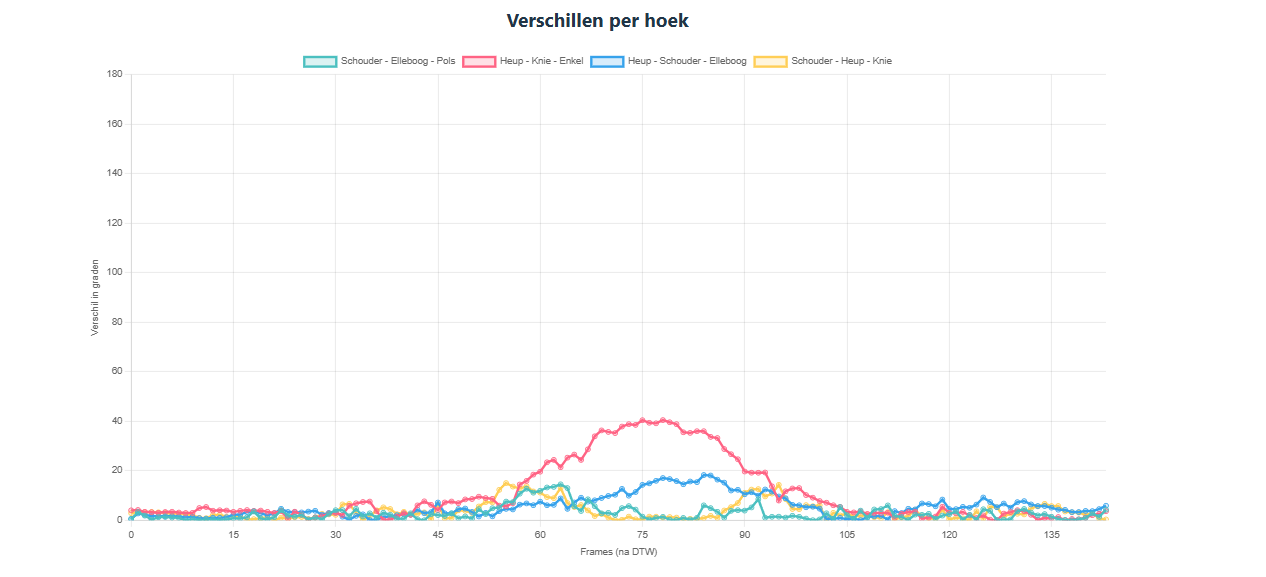
\includegraphics[width=0.9\textwidth]{deadlift_bad_back.png}
\caption{Hoekverschillen bij deadlift met foute rugpositie}
\label{fig:deadlift_bad_back}
\end{figure}

\section{Squat}
\subsection{Foute rugpositie tijdens squat}

Figuur~\ref{fig:squat_bad_back} toont de hoekverschillen bij een squat waarbij de rug onvoldoende recht wordt gehouden. 
We zien dat vooral de heup-knie-enkel-hoek (roze lijn) en de schouder-heup-knie-hoek (gele lijn) abnormale schommelingen vertonen rond het midden van de beweging (frames 60–90). 
Dit wijst op een instabiele rompcontrole.
Ook de heup-schouder-elleboog-hoek (blauwe lijn) vertoont een kleine piek, wat suggereert dat de bovenlichaampositie verandert om te compenseren voor de kromming van de rug. 
Deze afwijkingen verhogen het risico op overbelasting van de rug.

\begin{figure}[H]
\centering
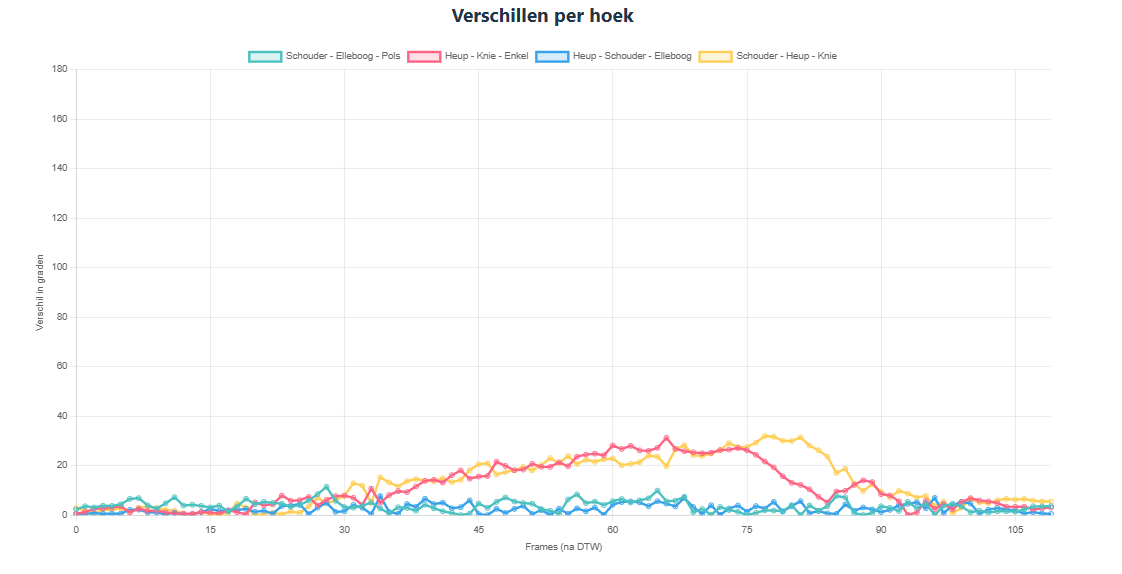
\includegraphics[width=0.9\textwidth]{squat_bad_back.png}
\caption{Hoekverschillen bij squat met gebogen rug}
\label{fig:squat_bad_back}
\end{figure}


\subsection{Te brede voetstand bij squat}

In Figuur~\ref{fig:squat_stance_wide} analyseren we een squat uitgevoerd met een te brede stand. 
Hier is opvallend dat de kniehoek (roze lijn) toeneemt rond frame 70, wat wijst op een overmatige spreiding van de benen. 

Daarnaast is de hoek tussen schouder-heup-knie (gele lijn) vrij stabiel, maar toch iets hoger dan bij een correcte uitvoering. De arm- en bovenlichaamhoeken blijven grotendeels neutraal. Deze positie kan leiden tot extra spanning op de lies en knieën, vooral bij beperkte heupmobiliteit, wat het risico op peesontstekingen of overbelasting verhoogt.

\begin{figure}[H]
\centering
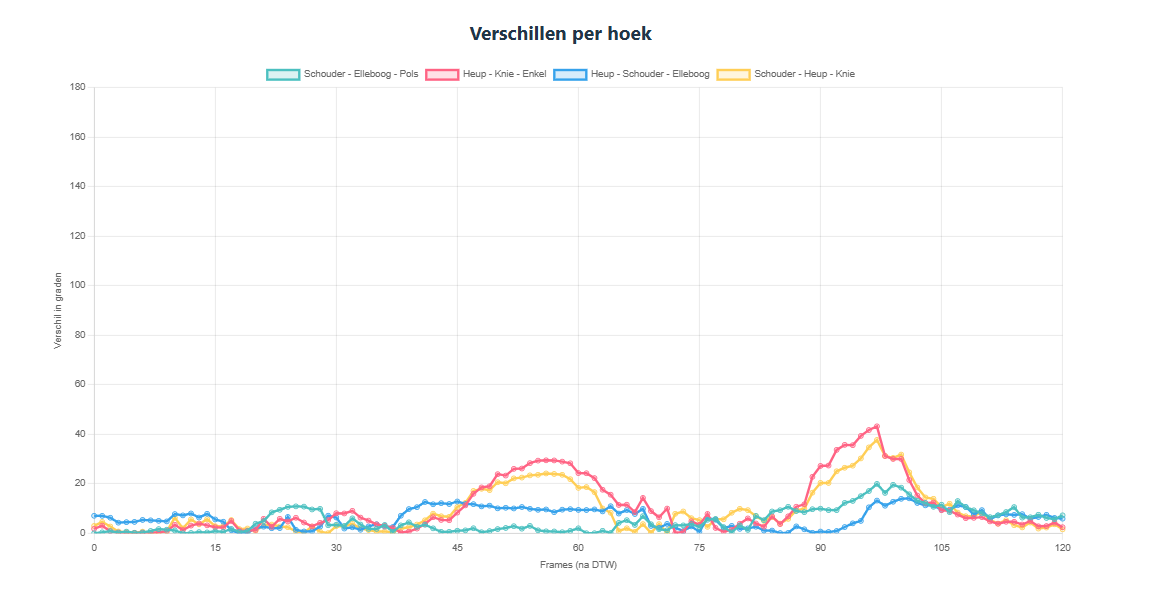
\includegraphics[width=0.9\textwidth]{squat_stance_too_wide.png}
\caption{Hoekverschillen bij squat met te brede voetstand}
\label{fig:squat_stance_wide}
\end{figure}

\section{Beperkingen van het algoritme}

Hoewel het algoritme ontworpen is om robuust te zijn voor variaties in lichaamsbouw, afstand tot de camera en uitvoeringssnelheid, zijn er toch enkele beperkingen waar rekening mee moet worden gehouden. 
Dit wordt duidelijk geïllustreerd in Figuur~\ref{fig:squat_same}, Figuur~\ref{fig:bench_same} en Figuur~\ref{fig:deadlift_same}, waarin exact dezelfde videofragmenten met zichzelf worden vergeleken.

Opvallend is dat de lijnen in deze grafieken — hoewel zeer klein — niet volledig plat zijn. 
Kleine hoekverschillen tot ongeveer 5 à 10 graden blijven zichtbaar, terwijl bij een ideale vergelijking de verschillen exact nul zouden moeten zijn. 
Dit kan verklaard worden door een aantal factoren:

\begin{itemize}
    \item \textbf{Niet-deterministische keypoint detectie:} De hoekwaarden worden berekend op basis van keypoints die door een pose estimation-model worden gedetecteerd. Deze modellen zijn gevoelig aan minieme variaties in belichting, ruis of compressie van het beeld, waardoor ze bij identieke inputframes toch licht verschillende coördinaten kunnen geven.
    
    \item \textbf{Interpolatie binnen Dynamic Time Warping:} Het DTW-algoritme rekt of comprimeert het tijdspad om een optimale uitlijning te bekomen. Zelfs bij twee identieke video’s kan het pad lichtjes afwijken door kleine numerieke onnauwkeurigheden of meerdere gelijke kostpaden. Daardoor kunnen frames die initieel identiek waren, toch aan net verschillende partnerframes gekoppeld worden.
    
    \item \textbf{Afwijkingen door ontbrekende of foutieve keypoints:} Bij sommige frames detecteert het model tijdelijk geen of foutieve gewrichtspunten, bijvoorbeeld door occlusie of een afwijkende houding. Hoewel het algoritme zulke frames uitsluit, kunnen korte storingen alsnog kleine schommelingen veroorzaken in de berekende gemiddelde verschillen.
    
    \item \textbf{Kwantificatiegevoeligheid bij hoeken:} De berekende hoeken zijn gevoelig aan afrondingen en kleine verschillen in de onderliggende vectorrichtingen. Omdat een hoek wordt bepaald op basis van drie punten, kan een afwijking van slechts enkele pixels al leiden tot een verschil van enkele graden.
\end{itemize}

In de praktijk zijn deze afwijkingen klein genoeg (minder dan 5–10 graden) om geen invloed te hebben op de interpretatie van fouten of afwijkingen in beweging. Wel is het belangrijk om deze limieten te kennen, vooral wanneer zeer kleine verschillen geïnterpreteerd worden.

\begin{figure}[H]
\centering
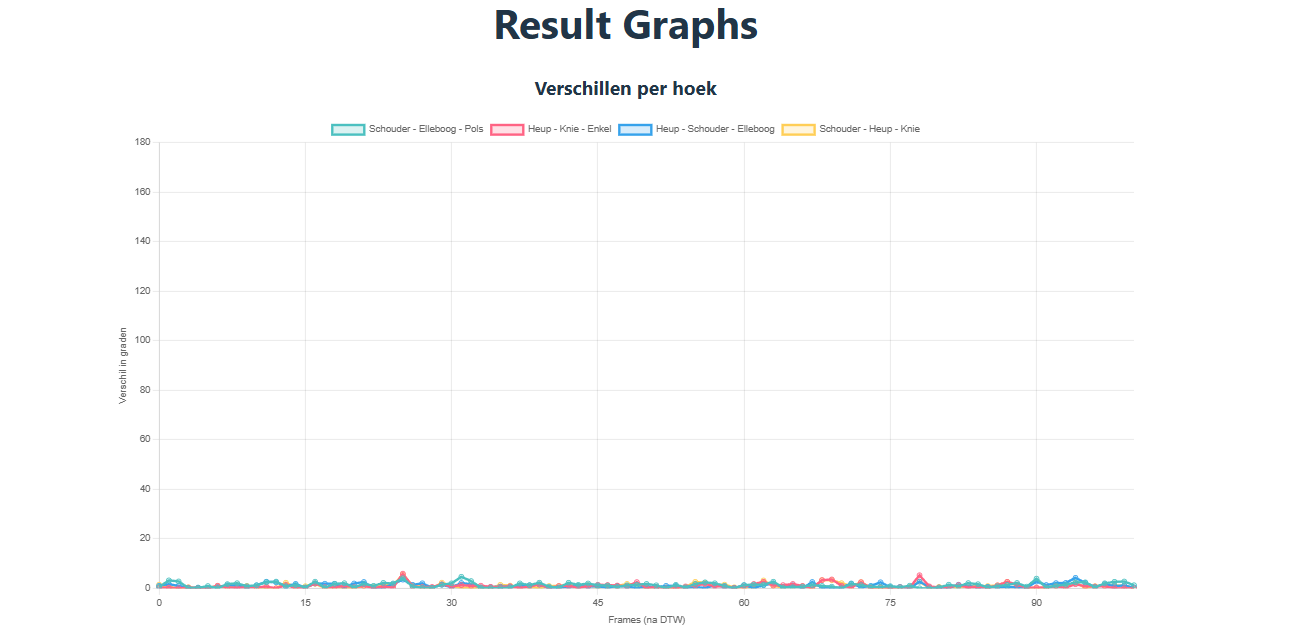
\includegraphics[width=0.9\textwidth]{squat_same_video.png}
\caption{Vergelijking van squatvideo met zichzelf}
\label{fig:squat_same}
\end{figure}

\begin{figure}[H]
\centering
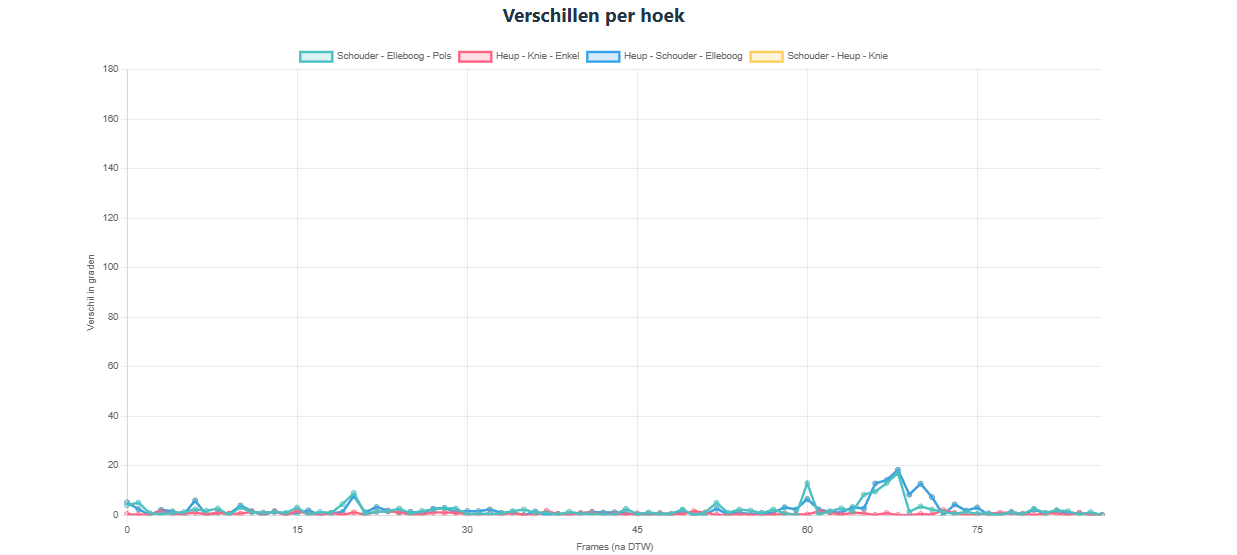
\includegraphics[width=0.9\textwidth]{bench_same_video.png}
\caption{Vergelijking van bench press video met zichzelf}
\label{fig:bench_same}
\end{figure}

\begin{figure}[H]
\centering
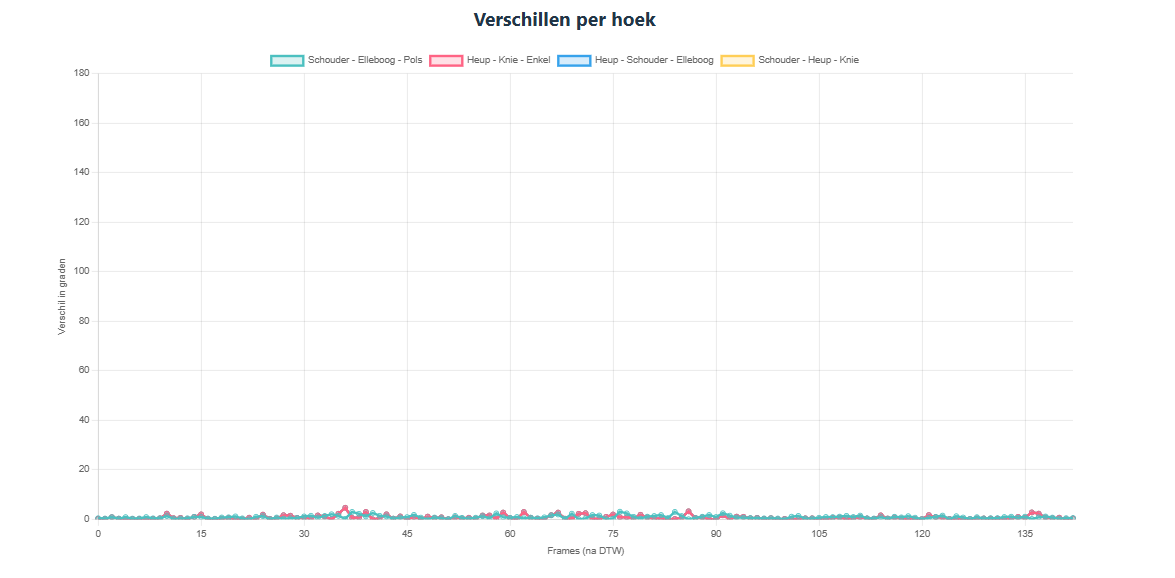
\includegraphics[width=0.9\textwidth]{deadlift_same_video.png}
\caption{Vergelijking van deadliftvideo met zichzelf}
\label{fig:deadlift_same}
\end{figure}

\section{Sterkte van het algoritme: robuustheid voor lichaamstype en camerahoek}

Een van de belangrijkste sterktes van het voorgestelde algoritme is de robuustheid voor verschillen in lichaamsbouw, lichaamslengte en afstand tot de camera. 
Deze eigenschap vloeit voort uit het feit dat het algoritme gebruikmaakt van \textbf{relatieve hoeken} tussen gewrichten in plaats van absolute pixelcoördinaten. 
Hierdoor wordt de analyse geschaald onafhankelijk van de afmetingen of positie van de gebruiker in het beeld.

\medskip

Figuur~\ref{fig:squat_diff_person}, Figuur~\ref{fig:bench_diff_person} en Figuur~\ref{fig:deadlift_diff_person} tonen telkens een vergelijking tussen een oefening uitgevoerd door twee verschillende personen met duidelijk verschillende lichaamsbouw. 
Ondanks deze verschillen blijven de hoekverschillen over het algemeen beperkt tot onder de 20 à 30 graden, wat aantoont dat het algoritme erin slaagt de algemene bewegingspatronen te detecteren, ongeacht individuele anatomie.

In de squatvergelijking (Figuur~\ref{fig:squat_diff_person}) zien we een korte verhoging in heup- en rompgerelateerde hoeken (gele en blauwe lijnen), mogelijk te wijten aan verschillende squatdiepte of voetpositie, maar zonder drastische afwijkingen.

\medskip

Voor de bench press (Figuur~\ref{fig:bench_diff_person}) blijven alle hoeken relatief stabiel, wat suggereert dat beide personen een gelijkaardige techniek hanteren ondanks anatomische verschillen.

\medskip

Bij de deadliftvergelijking (Figuur~\ref{fig:deadlift_diff_person}) valt vooral de blauwe lijn (Heup–Schouder–Elleboog) op, die een afwijking toont tussen frame 30 en 80. Dit wijst op een verschil in bovenlichaamhelling, maar de overige hoeken blijven consistent, wat wijst op een globale vergelijkbaarheid van de techniek.

\medskip

Deze resultaten bevestigen dat het algoritme in staat is om relevante biomechanische vergelijkingen te maken zonder dat voorafgaande kalibratie of persoonspecifieke normalisatie nodig is.

\begin{figure}[h]
\centering
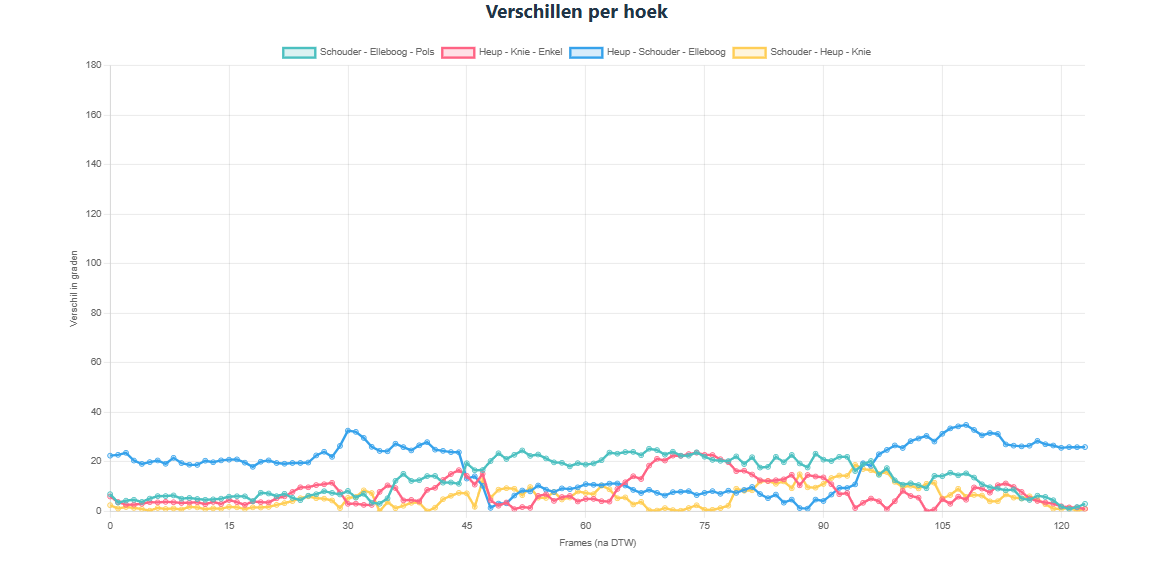
\includegraphics[width=0.9\textwidth]{squat_different_person.png}
\caption{Vergelijking van squat tussen twee personen met verschillende lichaamsbouw}
\label{fig:squat_diff_person}
\end{figure}

\begin{figure}[h]
\centering
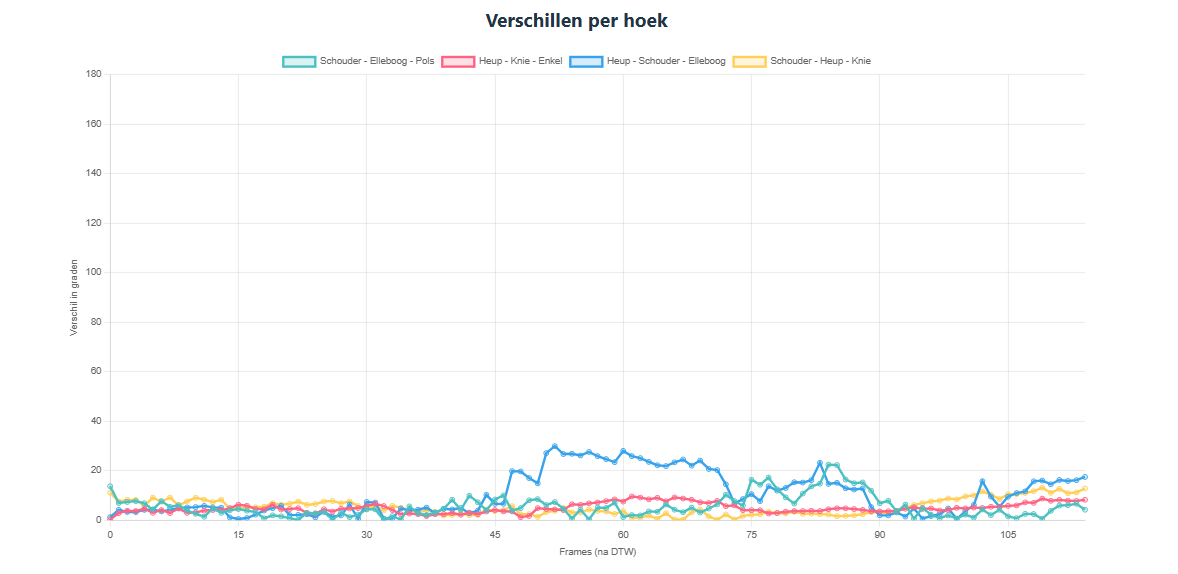
\includegraphics[width=0.9\textwidth]{bench_different_person.png}
\caption{Vergelijking van bench press tussen twee personen met verschillende lichaamsbouw}
\label{fig:bench_diff_person}
\end{figure}

\begin{figure}[h]
\centering
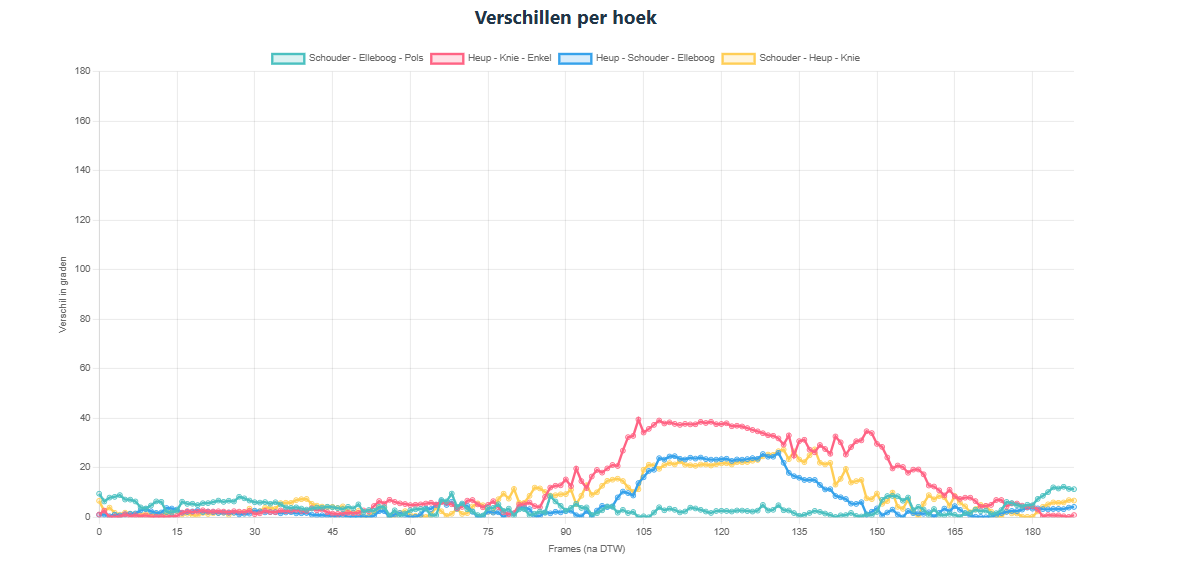
\includegraphics[width=0.9\textwidth]{deadlift_different_person.png}
\caption{Vergelijking van deadlift tussen twee personen met verschillende lichaamsbouw}
\label{fig:deadlift_diff_person}
\end{figure}


